\documentclass[../dissertation]{subfiles}

\begin{document}
\subsubsection{Conceptual Dependencies and Predicate-Argument structures}

\textbf{Primitives}

For each Conceptual Dependency primitive we will now list logical conclusions which can be drawn from the slots in the event.

\begin{description}
\item[PTRANS]\hfill

Required Arguments:

\begin{itemize}
\item Actor
\item Object \textit{Should default to Actor if unset}
\item Direction
\end{itemize}

Before event:
\[Location(Object) = \textit{Direction.Before}\]

After event:
\[Location(Object) = \textit{Direction.After}\]


\item[MOVE]\hfill

Required Arguments
\begin{itemize}
\item Actor
\item Object \textit{Must be part of actor}
\end{itemize}

Before event:
\[Location(Object) = \textit{Direction.Before}\]

After event:
\[Location(Object) = \textit{Direction.After}\]

\item[PROPEL]\hfill

Required Arguments
\begin{itemize}
	\item Actor
    \item Object
    \item Direction
    \begin{itemize}
    	\item Before
        \item After
    \end{itemize}
\end{itemize}

Before event:
\[Location(Object) = \textit{Direction.Before}\]

After event:
\[Velocity(Object) \propto \textit{Direction.After} - \textit{Direction.Before}\]

\item[EXPEL]\hfill

Required Arguments
\begin{itemize}
	\item Actor
    \item Object
\end{itemize}

Before event:
\[inside(Object, Actor)\]

After event:
\[NOT(inside(Object, Actor))\]

\item[INJEST]\hfill

Required Arguments
\begin{itemize}
	\item Actor
    \item Object
\end{itemize}


Before event:
\[NOT(inside(Object, Actor))\]

After event:
\[inside(Object, Actor)\]
\end{description}

\newpage

\textbf{Verbs}

We will now list a series of example verbs in terms of their CD primitives, with some slots filled in.

\textbf{Emit}

\smallskip

\begin{center}
	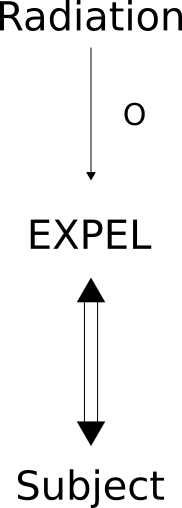
\includegraphics[height=200pt]{emit-cd.png}
\end{center}

Event Sequence
\begin{center}

    \begin{tabular}{l l}
      \toprule
      \multicolumn{2}{l}{\textbf{EXPEL event}}\\
      \hline
      \textbf{Actor:} & \textit{Subject}\\
      \textbf{Object:} & \textit{Object}\\
      \bottomrule
    \end{tabular}
\end{center}

Natural Language Example

\textit{The star emits radiation}

\textit{Subject:} Star

\textit{Object:} Radiation

\bigskip
\textit{Predicate/Argument inferences}

Before event:
\[inside(Radiation, Star)\]

After event:
\[NOT(inside(Radiation, Star))\]

\newpage %CHECK: NEW PAGE?

\textbf{Collapse}
\begin{center}
	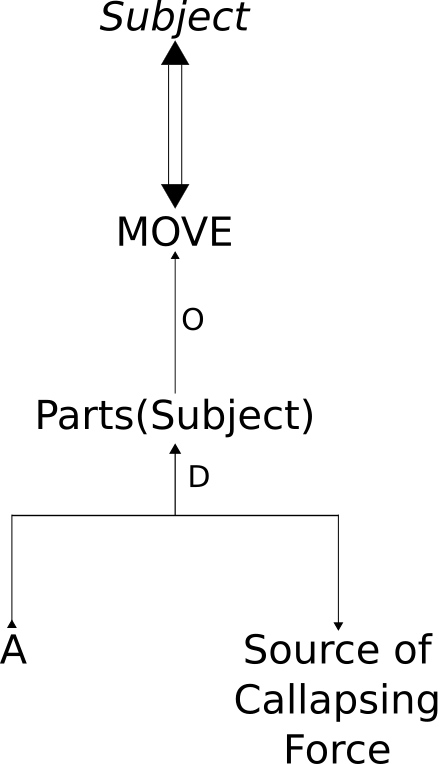
\includegraphics[height=200pt]{collapse-cd.png}
\end{center}
	\bigskip
    
Event Sequence
\begin{center}
    \begin{tabular}{l l}
      \toprule
      \multicolumn{2}{l}{\textbf{MOVE event}}\\
      \hline
      \textbf{Actor:} & \textit{Subject}\\
      \textbf{Object:} & Parts(\textit{Subject})\\
      
      \multicolumn{2}{l}{\textbf{Direction:}} \\
      Before: & \(A\) \\
      After: & \(Source of force\) \\
      \bottomrule
    \end{tabular}
    
\end{center}

Natural Language Example

\textit{The white dwarf collapses.}

\textit{Subject:} white dwarf

\textit{Object:} Parts of white dwarf \textit{from verb definition}

\bigskip

\textit{Predicate/Argument Inferences}

% \begin{tabular}{p{5cm} p{5cm}}
%   \toprule
%   Before & After \\
%   \midrule
%    Each part of white dwarf is at location \(A\)
%    & Each part of white dwarf is at the source of the collapsing force\\
%   \bottomrule
% \end{tabular}

Before event:
\[Location(Parts(Subject)) = A\]

After event:
\[Location(Parts(Subject)) = Source of force\]
\newpage

\textbf{Fall}

\bigskip
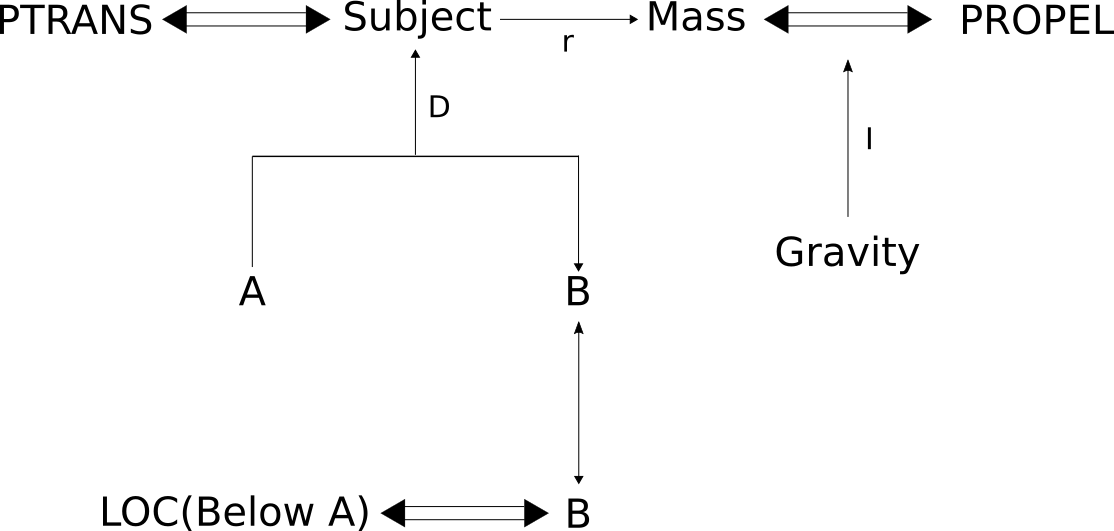
\includegraphics[width=\linewidth]{fall-cd.png}


Event Sequence

\begin{center}
  \begin{tabular}{l l}
  \toprule
  \multicolumn{2}{l}{\textbf{PROPEL event}}\\
  \hline
  \textbf{Actor:} & Mass\\
  \textbf{Object:} & \textit{Subject}\\
	\bottomrule
  \end{tabular}
  
  \smallskip
  results in
  \smallskip
  
  \begin{tabular}{l l}
    \toprule
    \multicolumn{2}{l}{\textbf{PTRANS event}}\\
    \hline
    \textbf{Actor:} & \textit{Subject}\\
    \multicolumn{2}{l}{\textbf{Direction:}} \\
    Before: & \(A\)\\
    After: & \(B = LOC(Below A)\)\\
    \bottomrule
  \end{tabular}
  
\end{center}

The ship fell into the black hole

\textit{Subject:} The ship

\textit{Object:} \textit{None}
\smallskip

\textit{Predicate/Argument inferences}

Event 1:

Before event:
\[Location(Ship) = A\]

After event:
\[Velocity(Ship) \propto Location(Mass) - A\]

Event 2:

Before event:
\[Location(Object) = A\]

After event:
\[Location(Object) = B\]
\bigskip

\textit{Notes:} While it is obvious the `mass' here is the black hole, this isn't captured by the logic presented here. If the sentence was `Jim fell into the pond', the pond isn't the gravity source- the planet he's standing on is!

The second half of the sentence, `\textit{into the black hole}' is a modifier for the verb phrase `\textit{The ship fell}'. To extend the logic presented here, the preposition `into' indicates the following location noun phrase takes the place of the `After' attribute of the PTRANS event's `Direction' attribute. This could be used to replace the variable \(B\) in the above diagrams.

In Propbank, this argument or modifier for the verb is labelled with a \textbf{GOL} role, which can be mapped to the Direction-After attribute in CD. This is further examined in Section~\ref{roles-to-slots}.
\newpage

\textbf{Reflect}

\textit{Constraints}
\textit{Object} is some form of Radiation moving towards \textit{Subject}
\bigskip

\begin{center}
	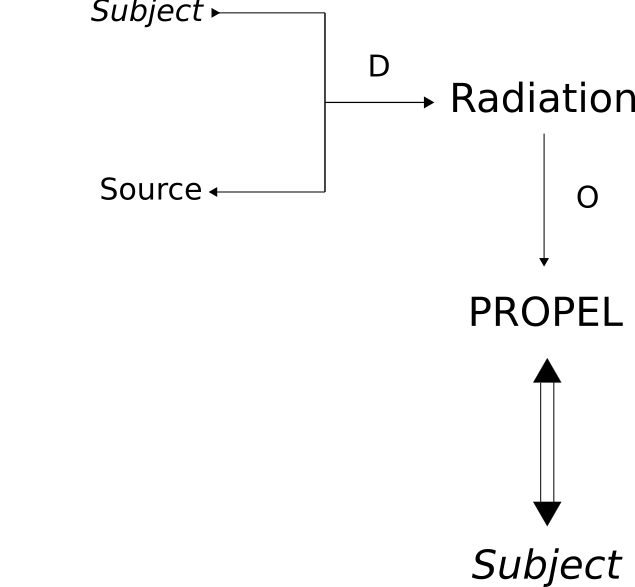
\includegraphics[height=200pt]{reflects-cd.png}
\end{center}

Event Sequence

\begin{center}
	
	\bigskip
    
    \begin{tabular}{l l}
      \toprule
      \multicolumn{2}{l}{\textbf{PROPEL event}}\\
      \hline
      \textbf{Actor:} & \textit{Subject}\\
      \textbf{Object:} & Radiation\\
      
      \multicolumn{2}{l}{\textbf{Direction:}} \\
      Before: & \textit{Subject}\\
      After: & Source\\
      \bottomrule
    \end{tabular}
    
\end{center}

Natural Language Example

\textit{The field reflects light}

\textit{Subject:} The field

\textit{Object:} light

\bigskip

Predicate-Argument Inferences

Before event:
\[Location(light) = field\]

After event:
\[Velocity(light) \propto Location(source) - Location(field)\]



% ========================
\textbf{Mapping Verb argument and modifier roles to CD slots}
\label{roles-to-slots}

Propbank and VerbNet are two online database of English verbs, which also list the semantic roles for 

\bigskip
\begin{table}
\begin{tabular}{l l l}
  \toprule
  CD Slot & Propbank Role & VerbNet Role \\
  \midrule
  Actor & Agent (PAG) & Agent\\
  Object & Patient (PTT) & Patient\\
  Direction: Before & Direction (DIR) & Source \\
  Direction: After &  Goal (GOL) & Destination \\
  \bottomrule
\end{tabular}
\caption{Alligning CD slots to semantic roles for verb arguments}
\end{table}
\end{document}